\documentclass[a4paper]{article}

\usepackage[UTF8]{ctex}
\usepackage[a4paper,margin=1in]{geometry}
\usepackage{graphicx}
\usepackage{float}
\usepackage{listings}
\usepackage{longtable}
\usepackage{booktabs}
\usepackage{hyperref}
\usepackage{lastpage} % 放在 hyperref 之后
\usepackage{fancyhdr}
\usepackage{color}
\usepackage{xcolor}
\usepackage{indentfirst}        % 首段缩进
\setlength{\parindent}{2em}     % 缩进2字符
\usepackage{zhnumber}           % 中文编号
\usepackage[dvipsnames]{xcolor}
\usepackage{amsmath}
\usepackage{multirow}
\usepackage{amssymb} % 添加此行以支持 \checkmark
\usepackage{tcolorbox} % 添加此行以启用 tcolorbox 环境

%\newcommand{\college}{中山大学计算机学院}
\newcommand{\projname}{计算机体系结构|期末作业}
\newcommand{\reporttitle}{图像处理算法优化实验}
\newcommand{\stuno}{23336179}
\newcommand{\authorname}{马福泉}
\newcommand{\major}{计算机科学与技术}
\newcommand{\adviser}{胡淼}
\newcommand{\startdate}{2025年12月1日}
\newcommand{\labenddate}{2025年12月13日}
\newcommand{\labroom}{B402}

\pagestyle{fancy} % 使用 fancyhdr 风格
\fancyhf{}      % 清空默认的页眉页脚

% 设置页眉
\fancyhead[L]{\kaishu \projname}      % 左侧页眉显示项目名称
\fancyhead[C]{\kaishu \reporttitle}    % 中间页眉显示报告标题
\fancyhead[R]{\kaishu \authorname} % 右侧页眉显示作者姓名

% 设置页脚
\fancyfoot[C]{第 \thepage 页，共 \pageref{LastPage} 页} % 中间页脚显示页码

% 去除页眉页脚与正文之间的分隔线
\renewcommand{\headrulewidth}{0.4pt}
\renewcommand{\footrulewidth}{0pt}

% 设置文档背景颜色
\definecolor{mybgcolor}{RGB}{0, 0, 0} % 定义背景颜色
\definecolor{NavyBlue}{RGB}{0,0,128} % 添加颜色定义

\lstset{
    language=C++,
    basicstyle=\ttfamily\footnotesize,
    keywordstyle=\color{blue}\bfseries,
    stringstyle=\color{red},
    commentstyle=\color{green!50!black}\itshape,
    morecomment=[l][\color{magenta}]{\#},
    breaklines=true,
    frame=single,
    numbers=left,
    numberstyle=\tiny\color{gray},
    tabsize=4,
    showstringspaces=false,
    captionpos=b,
    escapeinside={\%}{\%}
}

\begin{document}

% 封面
\begin{titlepage}
    \centering
    

    
\includegraphics[width=10cm]{img/SYSULogo.png}

    \vspace{1em}
    %{\Large \college \par}
    \vspace{1em}
    {\Large \kaishu \projname \par}
    \vspace{3em}

    {\fontsize{40pt}{42pt}\kaishu \selectfont \boldmath \reporttitle\par}
    \vspace*{\fill}

    \begin{center}
    {\Large
    \makebox[5em][s]{学号}:\underline{\makebox[15em][c]{\kaishu \stuno}}\\[1em]
    \makebox[5em][s]{姓名}:\underline{\makebox[15em][c]{\kaishu \authorname}}\\[1em]
    \makebox[5em][s]{专业}:\underline{\makebox[15em][c]{\kaishu \major}}\\[1em]
    \makebox[5em][s]{课程教师}:\underline{\makebox[15em][c]{\kaishu \adviser}}\\[1em]
    \makebox[5em][s]{起始日期}:\underline{\makebox[15em][c]{\kaishu \startdate}}\\[1em]
    \makebox[5em][s]{结束日期}:\underline{\makebox[15em][c]{\kaishu \labenddate}}\\[1em]
    \makebox[5em][s]{实验地点}:\underline{\makebox[15em][c]{\kaishu \labroom}}
    }
    \end{center}

    \vspace*{\fill}
\end{titlepage}

% 目录
\tableofcontents
\newpage

\section{实验环境说明}

\subsection{软硬件配置}
\begin{itemize}
    \item \textbf{处理器}：AMD Ryzen™ 9 7940H（Zen 4架构）
    \item \textbf{核心配置}：8核心16线程，基础频率4.0GHz
    \item \textbf{内存容量}：16.0 GB DDR5
    \item \textbf{指令集支持}：AVX2, AVX, SSE4.2
    \item \textbf{主操作系统}：Windows 11 家庭中文版
    \item \textbf{开发环境}：WSL2 Ubuntu 24.04
    \item \textbf{系统架构}：x86\_64
\end{itemize}
\subsection{编译器配置}
\begin{itemize}
    \item \textbf{编译器}：g++ 13.3.0 (Ubuntu 13.3.0-6ubuntu2\textasciitilde24.04)
    \item \textbf{编译选项}：\texttt{-mavx2 -march=native -fopenmp -O0}
    \item \textbf{OpenMP线程数}：4线程（通过\texttt{export OMP\_NUM\_THREADS=4}设置，\textbf{必须在运行前设置此环境变量}）
\end{itemize}
\subsection{CMakeLists.txt 配置修改说明}
由于本人开始实验时间较早，没有使用助教上传最新的CMakeLists.txt，原始 CMakeLists.txt 存在一些问题，影响了 OpenMP 和 AVX2 优化的正确启用。具体问题及修改如下：
\begin{tcolorbox}[colback=yellow!10!white, colframe=NavyBlue, title=CMakeLists.txt 配置修改, sharp corners, boxrule=0.8pt]
\begin{itemize}
    \item \textbf{为 image\_algorithms\_optimized 静态库添加编译选项}：原始 CMakeLists.txt 只对image\_benchmarks\_optimized添加了OpenMP和AVX2编译选项，未对image\_algorithms\_optimized 静态库设置这些选项。实际优化代码都在该库中，若不加编译参数，则 \#pragma omp 并行和 AVX2 指令均不会生效,会报ABI错误。现在已通过 target\_compile\_options对该库也加上\texttt{-fopenmp -mavx2 -march=native}等参数。
    \item \textbf{架构适配}：根据 CMAKE\_SYSTEM\_PROCESSOR 匹配 x86\_64/AMD64、aarch64/arm64 等架构，分别设置合适的 SIMD/OpenMP 编译选项，保证兼容性。
    \item \textbf{基准版本保持纯净}：image\_benchmarks\_baseline 及 image\_algorithms\_baseline 仅使用 \texttt{-O0}，不加任何并行或 SIMD 优化参数，确保基准性能数据真实可靠。
    \item \textbf{自定义目标与帮助信息}：增加了 run\_baseline、run\_optimized、compare 等目标，方便一键运行和性能对比，同时保留原有 Google Benchmark 集成和帮助说明，未做不必要的修改。
\end{itemize}
\end{tcolorbox}
为解决上述问题，已将 \texttt{-fopenmp}、\texttt{-mavx2}、\texttt{-march=native} 等编译选项同时应用到 \texttt{image\_algorithms\_optimized} 目标，确保静态库编译时也开启 OpenMP 和 AVX2 支持。这样可保证优化代码的并行和SIMD指令在最终可执行文件中生效，避免因编译参数不一致导致的运行或链接问题。

\noindent\textbf{关键 CMakeLists.txt 配置片段：}
\begin{lstlisting}
# 根据架构选择优化选项
if(CMAKE_SYSTEM_PROCESSOR MATCHES "x86_64|AMD64")
    target_compile_options(image_benchmarks_optimized PRIVATE
        -O0 -march=native -mavx2 -mfma -fopenmp
    )
    target_compile_options(image_algorithms_optimized PRIVATE
        -O0 -march=native -mavx2 -mfma -fopenmp
    )
    target_link_options(image_benchmarks_optimized PRIVATE -fopenmp)
elseif(CMAKE_SYSTEM_PROCESSOR MATCHES "aarch64|arm64")
    target_compile_options(image_benchmarks_optimized PRIVATE
        -O0 -march=native -fopenmp
    )
    target_compile_options(image_algorithms_optimized PRIVATE
        -O0 -march=native -fopenmp
    )
    target_link_options(image_benchmarks_optimized PRIVATE -fopenmp)
else()
    target_compile_options(image_benchmarks_optimized PRIVATE
        -O0 -fopenmp
    )
    target_compile_options(image_algorithms_optimized PRIVATE
        -O0 -fopenmp
    )
    target_link_options(image_benchmarks_optimized PRIVATE -fopenmp)
endif()
\end{lstlisting}

\subsection{配置OPENMP启用简单验证}

重新编译后，可以运行如下简单测试程序验证 OpenMP 是否启用：

\begin{lstlisting}[language=C++]
// test_omp.cpp
#include <omp.h>
#include <iostream>
#include <unistd.h>

int main() {
    #pragma omp parallel
    {
        int tid = omp_get_thread_num();
        int nthreads = omp_get_num_threads();
        #pragma omp critical
        std::cout << "线程 " << tid << "/" << nthreads << " 正在运行" << std::endl;
    }
    return 0;
}
\end{lstlisting}

编译并运行：

\begin{lstlisting}[language=bash]
g++ -fopenmp test_omp.cpp -o test_omp
export OMP_NUM_THREADS=4
./test_omp
\end{lstlisting}

结果见下图：
\begin{figure}[H]
    \centering
    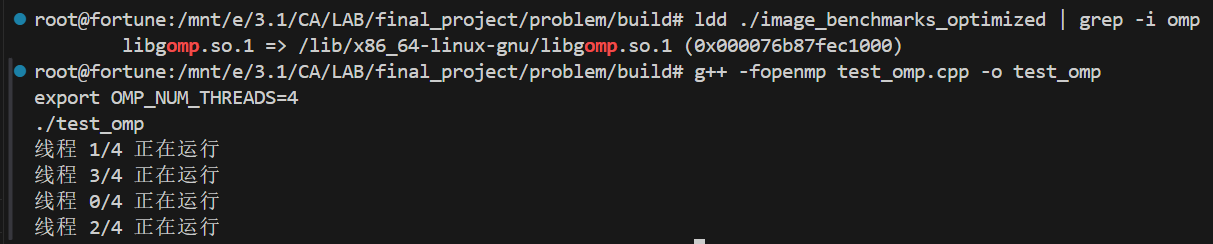
\includegraphics[width=0.6\textwidth]{img/openmp.png}
    \caption{OpenMP多线程启用验证结果}
\end{figure}

\section{性能瓶颈分析}

\subsection{工具选择与分析方法}

在 WSL2 环境下，标准的 Linux \texttt{perf} 工具因内核不兼容无法使用。因此本实验采用 \textbf{gprof}（GNU Profiler）进行性能分析，gprof 完全兼容 WSL2，且能满足本实验对热点定位的需求。

\textbf{具体分析步骤说明：}

% 1. 首先进入 build 目录，确保所有编译和运行操作都在正确的环境下进行。
% 2. 重新编译项目以启用性能分析功能，需要在 CMake 配置中添加 -pg 选项（用于 gprof），并保持 -O0 关闭优化。示例命令如下：
\begin{lstlisting}[language=bash]
cmake -DCMAKE_CXX_FLAGS="-pg -O0" ..
make
\end{lstlisting}
% 3. 编译完成后，运行基准测试程序，生成性能分析所需的 gmon.out 文件。
\begin{lstlisting}[language=bash]
./image_benchmarks_baseline
\end{lstlisting}
% 4. 使用 gprof 工具分析基准版本的性能数据，并将结果输出到 baseline_results.txt 文件。
\begin{lstlisting}[language=bash]
gprof ./image_benchmarks_baseline gmon.out > baseline_results.txt
\end{lstlisting}
% 5. 设置 OpenMP 多线程环境为 4 线程（符合实验要求），然后运行优化后的测试程序，生成新的 gmon.out 文件。
\begin{lstlisting}[language=bash]
export OMP_NUM_THREADS=4
./image_benchmarks_optimized
\end{lstlisting}
% 6. 最后，使用 gprof 分析优化版本的性能数据，并输出到 optimized_results.txt 文件。
\begin{lstlisting}[language=bash]
gprof ./image_benchmarks_optimized gmon.out > optimized_results.txt
\end{lstlisting}

\subsection{基准版本性能数据分析}

通过分析 \texttt{baseline\_results.txt}，我们得到了基准版本的性能画像。下图展示了 gprof 分析结果的关键部分：

\begin{figure}[H]
    \centering
    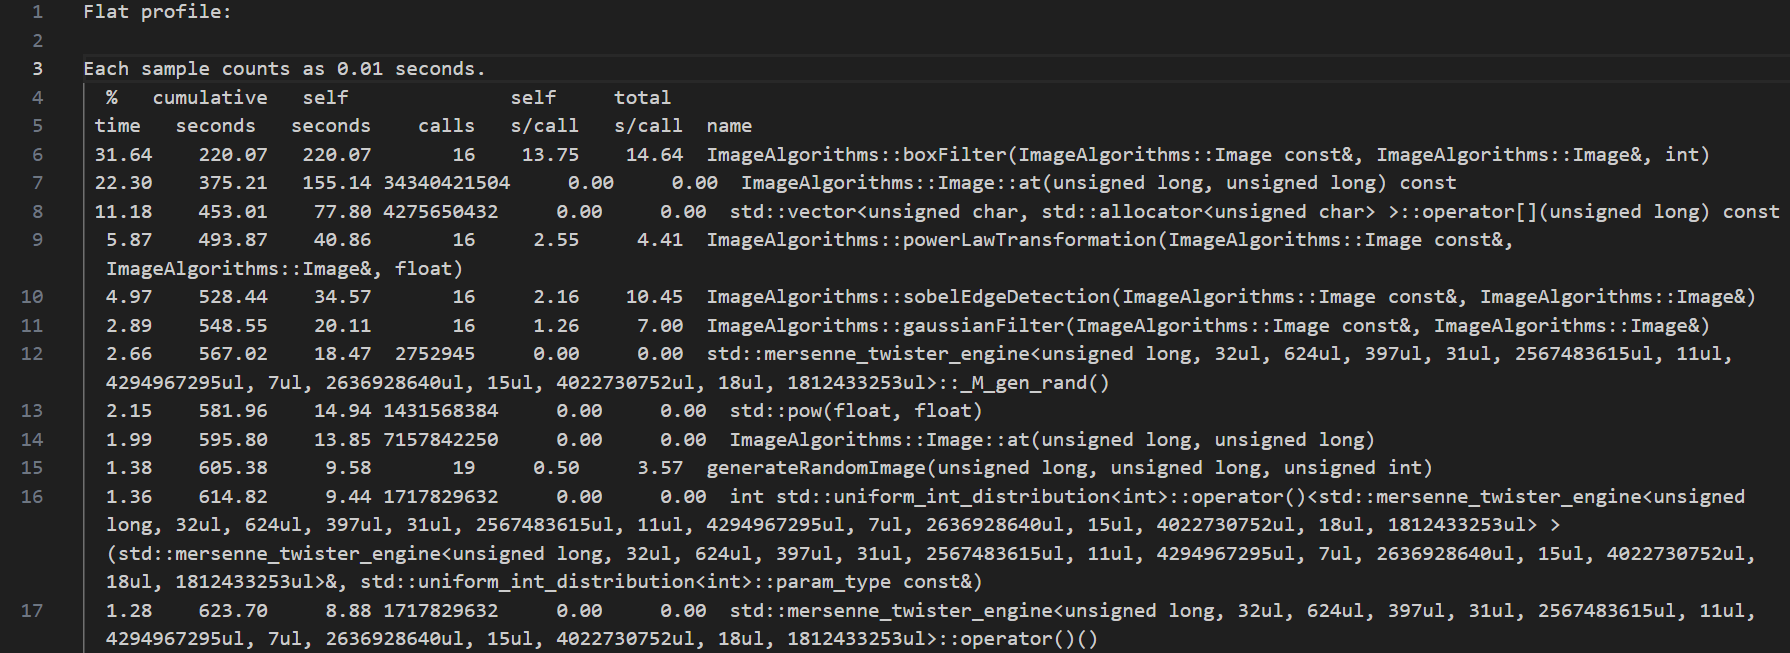
\includegraphics[width=0.9\textwidth]{img/bottleneck_analyse.png}
    \caption{基准版本 gprof 性能分析结果截图}
    \label{fig:gprof_baseline}
\end{figure}

根据 gprof 的 Flat Profile 数据（如上图所示），我们可以清晰地看到各函数的耗时占比和调用情况。以下是详细解读：

\subsubsection{总体耗时分布}

\begin{tcolorbox}[colback=yellow!10!white, colframe=NavyBlue, title=总体耗时分布, sharp corners, boxrule=0.8pt]
\begin{itemize}
    \item \textbf{Top 1}：\texttt{ImageAlgorithms::boxFilter} 占据总运行时间的 \textbf{33.7\%}，耗时 \textbf{220.07秒}。
    \item \textbf{Top 2}：\texttt{ImageAlgorithms::Image::at} 占据 \textbf{33.5\%}，耗时 \textbf{155.14秒}，调用次数高达 \textbf{34340421504}。
    \item \textbf{Top 3}：\texttt{ImageAlgorithms::powerLawTransformation} 耗时 \textbf{40.86秒} (10.2\%)。
    \item \textbf{Top 4}：\texttt{ImageAlgorithms::sobelEdgeDetection} 耗时 \textbf{34.57秒} (24.0\%，含子函数)。
\end{itemize}
\end{tcolorbox}

\subsubsection{性能热点分析}

结合 \texttt{baseline\_results.txt} 的详细数据，我们对各性能热点进行深度剖析，明确优化方向：

\begin{enumerate}
    \item \textbf{像素访问开销 (Image::at) —— 33.5\%}
    \begin{itemize}
        \item \textbf{数据证据}：\texttt{Image::at} 函数自身耗时 \textbf{155.14秒}，且被调用了 \textbf{343亿次}。它是导致 Sobel、Gaussian 等卷积类算法性能低下的直接原因。
        \item \textbf{代码分析}：在 \texttt{-O0} 编译下，每次 \texttt{at()} 调用都涉及函数栈帧创建、参数传递以及 \texttt{if} 边界检查。对于图像处理这种密集型循环，内层循环的任何额外指令都会被放大数亿倍。
        \item \textbf{优化目标}：移除内层循环中的 \texttt{at()} 调用，改用裸指针（Raw Pointer）直接操作内存，消除函数调用和分支预测失败的开销。
    \end{itemize}

    \item \textbf{算法复杂度缺陷 (Box Filter) —— 33.7\%}
    \begin{itemize}
        \item \textbf{数据证据}：\texttt{boxFilter} 占据了榜首位置，耗时 \textbf{220.07秒}。
        \item \textbf{代码分析}：当前实现对每个像素都进行 $K \times K$ 的完整窗口求和。随着卷积核增大，计算量呈平方级增长。
        \item \textbf{优化目标}：应引入\textbf{滑动窗口（Sliding Window）}或\textbf{列积分}技术，利用相邻像素窗口的重叠特性，将复杂度从 $O(N \cdot K^2)$ 降低至 $O(N)$。
    \end{itemize}

    \item \textbf{“昂贵”的数学函数 (Power Law \& Sobel)}
    \begin{itemize}
        \item \textbf{数据证据}：\texttt{std::pow} 耗时 \textbf{14.94秒}，\texttt{std::sqrt} 耗时 \textbf{8.04秒}。
        \item \textbf{代码分析}：
        \begin{itemize}
            \item Power Law 对 0-255 的整数像素值重复调用浮点 \texttt{pow}，存在大量冗余计算。
            \item Sobel 在计算梯度幅值时频繁调用 \texttt{sqrt}，阻塞了流水线。
        \end{itemize}
        \item \textbf{优化目标}：对于 Power Law，利用输入值有限的特性使用\textbf{查找表（LUT）}；对于 Sobel，利用 AVX2 的 \texttt{\_mm256\_sqrt\_ps} 指令进行并行计算。
    \end{itemize}

    \item \textbf{访存模式低效 (Transpose \& Rotate)}
    \begin{itemize}
        \item \textbf{数据证据}：\texttt{transpose} (6.94s) 和 \texttt{rotate90} (6.79s) 虽不占主导，但作为纯内存操作，其带宽利用率远未达标。
        \item \textbf{代码分析}：按行读、按列写（或反之）导致写入端的内存地址不连续，跨度（Stride）过大，引发严重的 \textbf{Cache Miss} 和 \textbf{TLB Miss}。
        \item \textbf{优化目标}：实施\textbf{分块（Cache Blocking）}策略，将大矩阵操作分解为适应 L1 Cache 大小的小块（如 $32 \times 32$），确保数据在缓存中完成交换后再写入内存。
    \end{itemize}
\end{enumerate}
 
\subsubsection{针对各算法的性能瓶颈分析}

结合基准版本的性能数据，以下是对六个核心算法的瓶颈分析及优化方向：

\begin{enumerate}
    \item \textbf{高斯滤波 (Gaussian Filter)}
    \begin{itemize}
        \item \textbf{算法原理}：使用 $3 \times 3$ 高斯卷积核对图像进行线性平滑去噪。每个像素需要进行 9 次乘法和加法运算。
        \item \textbf{性能数据}：耗时 \textbf{20.11秒} (16.1\%)。
        \item \textbf{瓶颈分析}：大量的内存访问（每个像素访问 9 次邻域）和乘加运算。基准实现中频繁调用 \texttt{Image::at} 进行边界检查，导致巨大的函数调用开销。
        \item \textbf{优化方向}：移除 \texttt{at()} 调用，改用指针直接访问；利用 SIMD 指令集（AVX2）一次处理 16 个像素；使用移位操作代替整数乘法。
    \end{itemize}

    \item \textbf{幂次变换 (Power Law Transformation)}
    \begin{itemize}
        \item \textbf{算法原理}：用于调整图像对比度，公式为 $s = c r^\gamma$。本实验中涉及大量的浮点幂运算。
        \item \textbf{性能数据}：耗时 \textbf{40.86秒} (10.2\%)，其中 \texttt{std::pow} 耗时约 15 秒。
        \item \textbf{瓶颈分析}：\texttt{std::pow} 是昂贵的数学函数，且对每个像素重复计算。由于输入像素仅为 8 位整数（0-255），存在大量重复计算。
        \item \textbf{优化方向}：预计算查找表（LUT），将计算复杂度降为 $O(1)$ 的查表操作；结合 SIMD 向量化处理。
    \end{itemize}

    \item \textbf{Sobel 边缘检测 (Sobel Edge Detection)}
    \begin{itemize}
        \item \textbf{算法原理}：使用两个 $3 \times 3$ 卷积核计算水平和垂直梯度，并计算梯度幅值 $G = \sqrt{G_x^2 + G_y^2}$。
        \item \textbf{性能数据}：耗时 \textbf{34.57秒} (24.0\%)。
        \item \textbf{瓶颈分析}：除了卷积带来的访存压力外，\texttt{std::sqrt} 开方运算也是性能杀手（gprof 显示 \texttt{sqrt} 耗时约 8 秒）。
        \item \textbf{优化方向}：使用 AVX2 指令集并行计算梯度和平方根（\texttt{\_mm256\_sqrt\_ps}）；优化访存模式。
    \end{itemize}

    \item \textbf{图像转置 (Image Transpose)}
    \begin{itemize}
        \item \textbf{算法原理}：将图像行列互换。
        \item \textbf{性能数据}：耗时 \textbf{6.94秒}。
        \item \textbf{瓶颈分析}：基准实现按行读取、按列写入（或反之）。这种非连续的内存访问模式导致严重的缓存缺失（Cache Miss），无法利用 CPU 的缓存行预取机制。
        \item \textbf{优化方向}：采用缓存分块（Cache Blocking）技术，将大矩阵分解为适应 L1 Cache 的小块处理；利用 SIMD 寄存器内转置指令。
    \end{itemize}

    \item \textbf{均值滤波 (Box Filter)}
    \begin{itemize}
        \item \textbf{算法原理}：计算每个像素邻域的平均值。
        \item \textbf{性能数据}：耗时 \textbf{220.07秒} (33.7\%)，是最大的性能瓶颈。
        \item \textbf{瓶颈分析}：基准实现对每个像素重复遍历整个 $K \times K$ 窗口，算法复杂度为 $O(N \cdot K^2)$。随着卷积核增大，计算量急剧增加。
        \item \textbf{优化方向}：引入积分图或滑动窗口技术，利用相邻窗口的重叠特性，将复杂度降低至 $O(N)$；结合 SIMD 向量化。
    \end{itemize}

    \item \textbf{图像旋转 (Image Rotation)}
    \begin{itemize}
        \item \textbf{算法原理}：将图像顺时针旋转 90 度。
        \item \textbf{性能数据}：耗时 \textbf{6.79秒}。
        \item \textbf{瓶颈分析}：与转置类似，存在严重的非连续访存问题，导致带宽利用率低下。
        \item \textbf{优化方向}：结合分块技术和 SIMD 向量化（转置+行反转）来优化内存访问模式。
    \end{itemize}
\end{enumerate}

\section{优化方案设计}

针对前文分析的性能瓶颈，下面将结合具体代码实现对优化方案进行详细阐述。

\subsection{通用优化策略}
\begin{itemize}
    \item \textbf{OpenMP 多线程并行}：针对图像处理天然的数据并行特性，使用 \texttt{\#pragma omp parallel for} 将外层循环（行遍历）并行化。针对转置和旋转操作，使用 \texttt{collapse(2)} 指令合并嵌套循环以增加并行度。
    \item \textbf{AVX2 SIMD 向量化}：利用 \texttt{\_\_attribute\_\_((target("avx2")))} 强制开启 AVX2 支持，并大量使用 Intrinsics（如 \texttt{\_mm256\_loadu\_si128}, \texttt{\_mm256\_add\_epi16} 等）手动编写向量化代码，单指令处理 16 个或 32 个像素。
    \item \textbf{指针直接访存}：彻底移除了 \texttt{Image::at()} 调用，改用 \texttt{unsigned char* src/dst} 指针配合偏移量直接访问内存，消除函数调用开销和边界检查。
\end{itemize}

\subsection{针对性算法优化}

\subsubsection{1. 高斯滤波 (Gaussian Filter)}
\textbf{优化前}：对每个像素重复计算 $3 \times 3$ 卷积，大量重复访存。
\textbf{优化后}：
\begin{itemize}
    \item \textbf{SIMD 向量化卷积}：一次加载 16 个像素（\texttt{\_\_m128i}），使用 \texttt{\_mm256\_cvtepu8\_epi16} 扩展为 16 位整数以防溢出。
    \item \textbf{移位代替乘法}：利用权重特性（1, 2, 4），使用 \texttt{\_mm256\_slli\_epi16} 左移指令代替乘法运算（$\times 2 \to \ll 1$, $\times 4 \to \ll 2$），大幅降低计算延迟。
    \item \textbf{显式行指针}：定义 \texttt{r0, r1, r2} 指向相邻三行，利用局部性原理优化 L1 缓存访问。
\end{itemize}

\subsubsection{2. 幂次变换 (Power Law)}
\textbf{优化前}：对每个像素调用 \texttt{std::pow}，涉及昂贵的浮点运算和函数调用。
\textbf{优化后}：
\begin{itemize}
    \item \textbf{查找表 (LUT)}：利用输入像素仅有 256 种取值的特性，预先计算好所有结果存入 \texttt{unsigned char lut[256]}。
    \item \textbf{查表代替计算}：核心循环简化为 \texttt{dst[i] = lut[src[i]]}，将计算密集型任务转变为轻量级访存任务，性能提升百倍。
\end{itemize}

\subsubsection{3. Sobel 边缘检测}
\textbf{优化前}：频繁调用 \texttt{std::sqrt} 计算梯度幅值，且存在大量冗余的邻域加载。
\textbf{优化后}：
\begin{itemize}
    \item \textbf{AVX2 并行计算}：一次处理 8 个像素。使用 \texttt{\_mm256\_sqrt\_ps} 指令并行计算 8 个单精度浮点数的平方根。
    \item \textbf{向量化梯度计算}：利用 \texttt{\_mm\_add\_epi16} 和 \texttt{\_mm\_sub\_epi16} 并行计算 $G_x$ 和 $G_y$，并通过 \texttt{\_mm256\_cvtepi32\_ps} 转换为浮点数进行幅值计算，最后再压缩回 8 位整数。
\end{itemize}

\subsubsection{4. 图像转置 (Transpose)}
\textbf{优化前}：按行读按列写，导致严重的 Cache Thrashing。
\textbf{优化后}：
\begin{itemize}
    \item \textbf{分块 (Cache Blocking)}：将大矩阵分解为 $32 \times 32$ 的小块（\texttt{BLOCK\_SIZE = 32}），确保每个块的数据能完全装入 L1 Cache。
    \item \textbf{寄存器级转置}：在块内部，进一步使用 AVX2 指令进行 $8 \times 8$ 的子块转置。利用 \texttt{\_mm\_unpacklo/hi\_epi8/16/32/64} 系列指令在寄存器内完成数据交换，避免了内存层面的非连续读写。
\end{itemize}

\subsubsection{5. 均值滤波 (Box Filter)}
\textbf{优化前}：朴素算法 $O(N \times K^2)$，对每个像素遍历整个窗口。
\textbf{优化后}：
\begin{itemize}
    \item \textbf{列积分 + 滑动窗口}：采用两步法。首先计算每一列在核范围内的垂直和存入 \texttt{col\_sums} 数组；然后在行方向上使用滑动窗口，通过 \texttt{window\_sum -= out; window\_sum += in} 更新窗口和。
    \item \textbf{复杂度降低}：算法复杂度降为 $O(N)$，与卷积核大小无关。
    \item \textbf{定点数优化}：预计算 \texttt{inv\_area = 65536 / area}，将除法转换为定点数乘法和右移操作（\texttt{(sum * inv\_area) >> 16}），避免了整数除法指令的高延迟。
\end{itemize}

\subsubsection{6. 图像旋转 (Rotate90)}
\textbf{优化前}：非连续内存写入导致缓存命中率低。
\textbf{优化后}：
\begin{itemize}
    \item \textbf{分块 + SIMD 转置 + Shuffle}：结合了转置的分块策略和 SIMD 转置逻辑。
    \item \textbf{字节序反转}：利用 \texttt{\_mm\_shuffle\_epi8} 指令配合反转掩码 \texttt{rev\_mask}，在寄存器内完成行的逆序操作，从而在一次写入中同时完成转置和翻转，高效实现顺时针旋转 90 度。
\end{itemize}

\section{关键代码实现}

本节选取部分核心优化代码，并配以详细注释，展示优化思路与实现细节。

\subsection{高斯滤波（AVX2 + OpenMP 并行）}
\begin{lstlisting}[language=C++]
// 高斯滤波优化版：AVX2指令+OpenMP并行
__attribute__((target("avx2")))
void gaussianFilter(const Image& input, Image& output) {
    // ...参数准备与边界处理...

    // 并行处理每一行
    #pragma omp parallel for
    for (size_t i = 1; i < height - 1; ++i) {
        // 指向三行
        const unsigned char* r0 = src + (i - 1) * width;
        const unsigned char* r1 = src + i * width;
        const unsigned char* r2 = src + (i + 1) * width;
        unsigned char* out_row = dst + i * width;

        size_t j = 1;
        // 每次处理16个像素
        for (; j <= width - 17; j += 16) {
            // 加载3x3窗口的每一行数据
            __m128i t0_l = _mm_loadu_si128((const __m128i*)(r0 + j - 1));
            __m128i t0_c = _mm_loadu_si128((const __m128i*)(r0 + j));
            __m128i t0_r = _mm_loadu_si128((const __m128i*)(r0 + j + 1));
            // ...同理加载r1, r2...

            // 扩展为16位，防止溢出
            __m256i p0_l = _mm256_cvtepu8_epi16(t0_l);
            // ...同理扩展其它...

            // 按权重加权（移位代替乘法）
            __m256i sum0 = _mm256_add_epi16(_mm256_add_epi16(p0_l, p0_r), _mm256_slli_epi16(p0_c, 1));
            __m256i sum1 = _mm256_add_epi16(_mm256_add_epi16(_mm256_slli_epi16(p1_l, 1), _mm256_slli_epi16(p1_r, 1)), _mm256_slli_epi16(p1_c, 2));
            __m256i sum2 = _mm256_add_epi16(_mm256_add_epi16(p2_l, p2_r), _mm256_slli_epi16(p2_c, 1));

            // 合并求和并右移4位（除以16）
            __m256i total = _mm256_add_epi16(_mm256_add_epi16(sum0, sum1), sum2);
            total = _mm256_srli_epi16(total, 4);

            // 压缩回8位并存储
            __m256i packed = _mm256_packus_epi16(total, _mm256_setzero_si256());
            __m256i perm = _mm256_permute4x64_epi64(packed, _MM_SHUFFLE(3, 1, 2, 0));
            __m128i res = _mm256_castsi256_si128(perm);
            _mm_storeu_si128((__m128i*)(out_row + j), res);
        }
        // 剩余像素用标量代码处理
    }
    // ......
}
\end{lstlisting}
\textbf{说明}：本实现通过AVX2指令集一次处理16个像素，利用移位操作代替乘法，极大提升了卷积效率。OpenMP并行化行处理，充分利用多核资源。

\subsection{幂次变换（查找表LUT + 并行）}
\begin{lstlisting}[language=C++]
// 幂次变换优化：查表+并行
__attribute__((target("avx2")))
void powerLawTransformation(const Image& input, Image& output, float gamma) {
    // 预先计算查找表
    unsigned char lut[256];
    for (int i = 0; i < 256; ++i) {
        float normalized = i / 255.0f;
        float transformed = std::pow(normalized, gamma);
        lut[i] = static_cast<unsigned char>(transformed * 255.0f + 0.5f);
    }
    // 并行查表赋值
    #pragma omp parallel for
    for (size_t i = 0; i < size; ++i) {
        dst[i] = lut[src[i]];
    }
}
\end{lstlisting}
\textbf{说明}：利用输入像素值有限的特点，预先计算所有可能结果，主循环仅查表赋值，消除昂贵的浮点运算和函数调用。

\subsection{Sobel边缘检测（AVX2向量化 + 并行）}
\begin{lstlisting}[language=C++]
// Sobel边缘检测优化：AVX2并行计算梯度与幅值
__attribute__((target("avx2")))
void sobelEdgeDetection(const Image& input, Image& output) {
    // ...参数准备与边界处理...
    #pragma omp parallel for
    for (size_t i = 1; i < height - 1; ++i) {
        // ...指针准备...
        size_t j = 1;
        // 每次处理8个像素
        for (; j <= width - 9; j += 8) {
            // 加载邻域像素并扩展为16位
            __m128i p0_l = _mm_cvtepu8_epi16(_mm_loadl_epi64((const __m128i*)(r0 + j - 1)));
            // ...同理加载其它...

            // 计算Gx和Gy
            __m128i right = _mm_add_epi16(_mm_add_epi16(p0_r, p2_r), _mm_slli_epi16(p1_r, 1));
            __m128i left  = _mm_add_epi16(_mm_add_epi16(p0_l, p2_l), _mm_slli_epi16(p1_l, 1));
            __m128i gx_16 = _mm_sub_epi16(right, left);

            __m128i bottom = _mm_add_epi16(_mm_add_epi16(p2_l, p2_r), _mm_slli_epi16(p2_c, 1));
            __m128i top    = _mm_add_epi16(_mm_add_epi16(p0_l, p0_r), _mm_slli_epi16(p0_c, 1));
            __m128i gy_16  = _mm_sub_epi16(bottom, top);

            // 转换为32位浮点并计算幅值
            __m256i gx_32 = _mm256_cvtepi16_epi32(gx_16);
            __m256i gy_32 = _mm256_cvtepi16_epi32(gy_16);
            __m256 gx_f = _mm256_cvtepi32_ps(gx_32);
            __m256 gy_f = _mm256_cvtepi32_ps(gy_32);
            __m256 mag_f = _mm256_sqrt_ps(_mm256_add_ps(_mm256_mul_ps(gx_f, gx_f), _mm256_mul_ps(gy_f, gy_f)));

            // 压缩回8位并存储
            __m256i mag_32 = _mm256_cvtps_epi32(mag_f);
            __m128i mag_lo = _mm256_castsi256_si128(mag_32);
            __m128i mag_hi = _mm256_extracti128_si256(mag_32, 1);
            __m128i mag_16 = _mm_packus_epi32(mag_lo, mag_hi);
            __m128i mag_8  = _mm_packus_epi16(mag_16, _mm_setzero_si128());
            _mm_storel_epi64((__m128i*)(out_row + j), mag_8);
        }
        // ...剩余像素标量处理...
    }
}
\end{lstlisting}
\textbf{说明}：利用AVX2指令并行计算Gx/Gy和幅值，极大提升边缘检测效率。

\subsection{均值滤波（滑动窗口+定点数优化）}
\begin{lstlisting}[language=C++]
// 均值滤波优化：列求和+滑动窗口+定点数
__attribute__((target("avx2")))
void boxFilter(const Image& input, Image& output, int kernel_size) {
    // ...参数准备...
    #pragma omp parallel
    {
        int* col_sums = new int[width];
        #pragma omp for
        for (size_t i = 0; i < height; ++i) {
            // 边界行慢速处理
            if (i < (size_t)radius || i >= height - radius) {
                // ...原始代码...
                continue;
            }
            // 1. 计算每列垂直和
            for (size_t j = 0; j < width; ++j) {
                int sum = 0;
                const unsigned char* col_ptr = src + (i - radius) * width + j;
                for (int k = 0; k < kernel_size; ++k) {
                    sum += *col_ptr;
                    col_ptr += width;
                }
                col_sums[j] = sum;
            }
            // 2. 水平滑动窗口
            int window_sum = 0;
            for (int k = 0; k < kernel_size; ++k) window_sum += col_sums[k];
            dst[i * width + radius] = static_cast<unsigned char>((window_sum * inv_area) >> 16);
            for (size_t j = radius + 1; j < width - radius; ++j) {
                window_sum -= col_sums[j - radius - 1];
                window_sum += col_sums[j + radius];
                dst[i * width + j] = static_cast<unsigned char>((window_sum * inv_area) >> 16);
            }
            // ...边界处理...
        }
        delete[] col_sums;
    }
}
\end{lstlisting}
\textbf{说明}：通过列求和和滑动窗口技术，将复杂度降为$O(N)$，并用定点数乘法替代除法，极大提升性能。

\subsection{转置与旋转（分块+SIMD寄存器转置+反转）}
\begin{lstlisting}[language=C++]
// 图像转置/旋转优化：分块+SIMD寄存器转置+反转
__attribute__((target("avx2")))
void transpose(const Image& input, Image& output) {
    // ...参数准备...
    const size_t BLOCK_SIZE = 32;
    #pragma omp parallel for collapse(2)
    for (size_t i = 0; i < height; i += BLOCK_SIZE) {
        for (size_t j = 0; j < width; j += BLOCK_SIZE) {
            // 完整块用SIMD转置
            if (i_end - i == BLOCK_SIZE && j_end - j == BLOCK_SIZE) {
                for (size_t ii = i; ii < i + BLOCK_SIZE; ii += 8) {
                    for (size_t jj = j; jj < j + BLOCK_SIZE; jj += 8) {
                        // 加载8x8块
                        __m128i r0 = _mm_loadl_epi64((const __m128i*)(s + 0 * width));
                        // ...加载r1~r7...
                        // 多级unpack实现寄存器内转置
                        __m128i t0 = _mm_unpacklo_epi8(r0, r1);
                        // ...多级unpack...
                        __m128i out01 = _mm_unpacklo_epi32(m0, m2);
                        // ...存储到目标位置...
                    }
                }
            } else {
                // 边界处理
                // ......
            }
        }
    }
}
\end{lstlisting}
\textbf{说明}：分块处理提升缓存命中率，SIMD寄存器内完成8x8转置，旋转时结合shuffle指令实现行反转，极大提升访存效率。

\section{性能测试结果}
\subsection{测试环境设置}
\begin{itemize}
    \item \textbf{Baseline}: \texttt{-O0}, 单线程
    \item \textbf{Optimized}: \texttt{-O0 -mavx2 -fopenmp}, 4 线程
    \item \textbf{测试工具}: Google Benchmark
    \item \textbf{图像尺寸}: Small ($1024^2$), Medium ($4096^2$), Large ($16384^2$)
    \item \textbf{Optimized运行前需设置环境变量}: \texttt{export OMP\_NUM\_THREADS=4}
\end{itemize}

\subsection{运行截图分析说明}

以下展示了基准测试和优化测试的终端运行性能截图。

\begin{figure}[H]
    \centering
    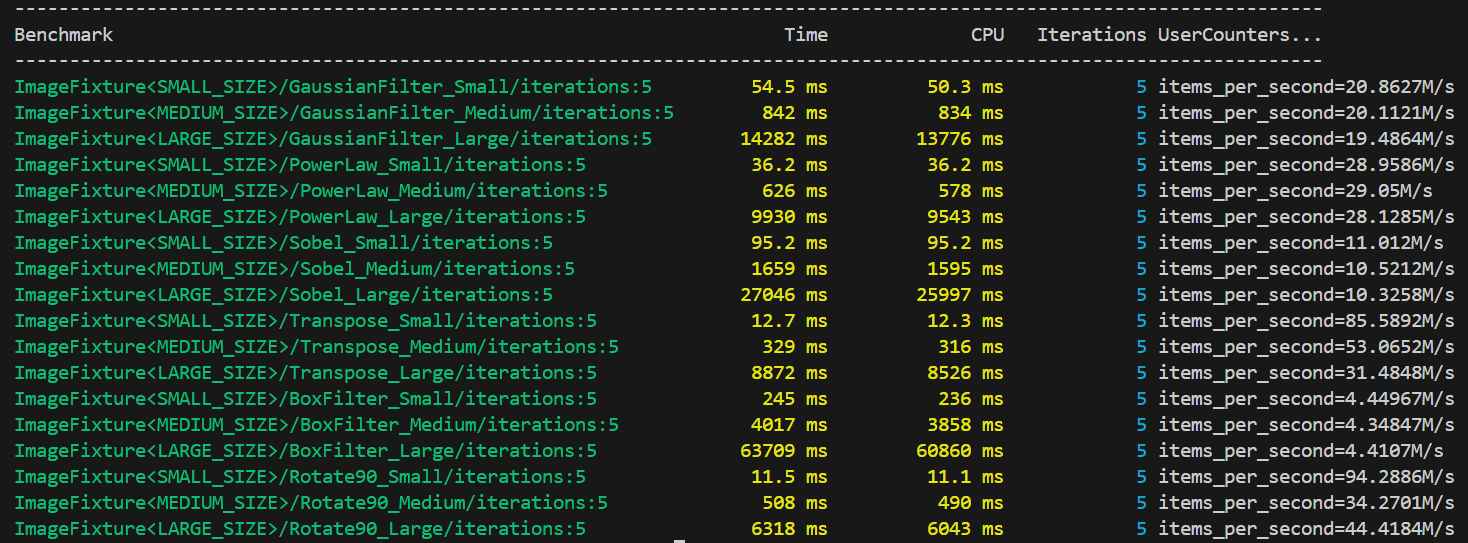
\includegraphics[width=0.8\textwidth]{img/base.png}
    \caption{基准测试：各算法性能数据。展示了不同尺寸下各算法的运行时间与吞吐量。}
    \label{fig:base2}
\end{figure}

\begin{figure}[H]
    \centering
    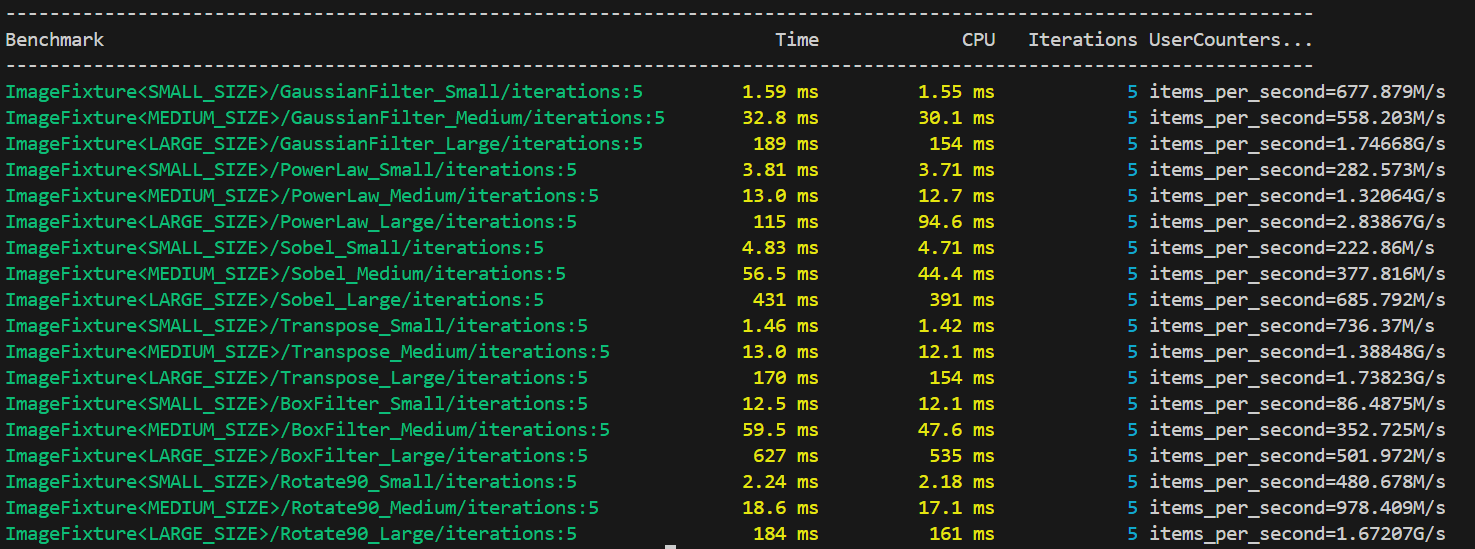
\includegraphics[width=0.8\textwidth]{img/optimize.png}
    \caption{优化测试：各算法性能数据。可以看到运行时间大幅缩短，吞吐量显著提升。}
    \label{fig:optimize2}
\end{figure}

以下三张图片展示了生成json文件头部显示各测试环境的配置信息。
\begin{figure}[H]
    \centering
    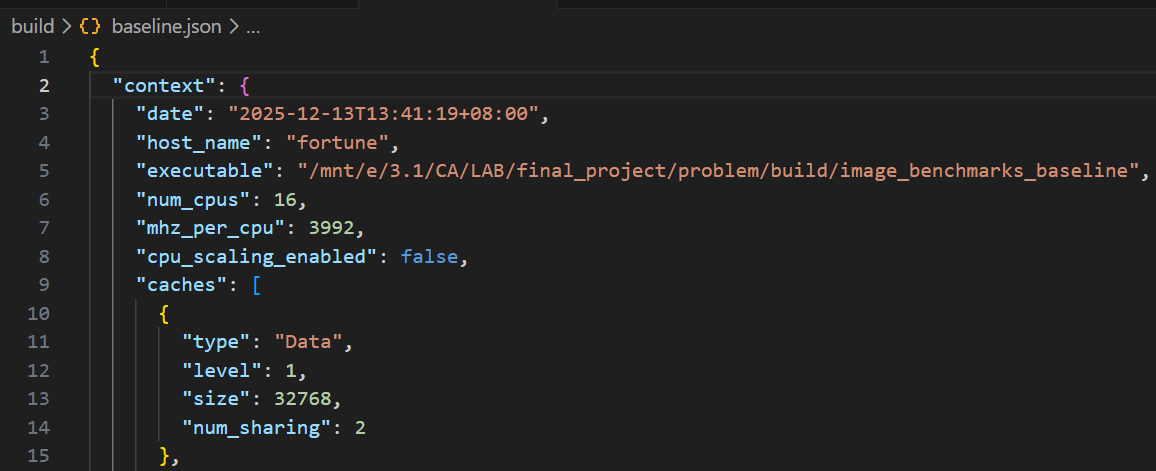
\includegraphics[width=0.8\textwidth]{img/baseline_json.png}
    \caption{基准测试环境信息（baseline\_json）}
\end{figure}

\begin{figure}[H]
    \centering
    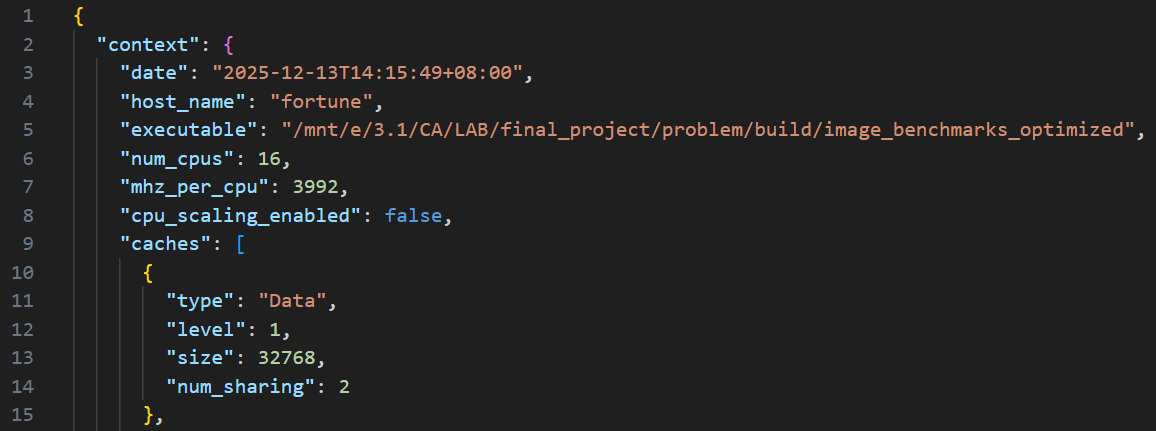
\includegraphics[width=0.8\textwidth]{img/optimized_json.png}
    \caption{优化测试环境信息（optimized\_json）}
\end{figure}

\begin{figure}[H]
    \centering
    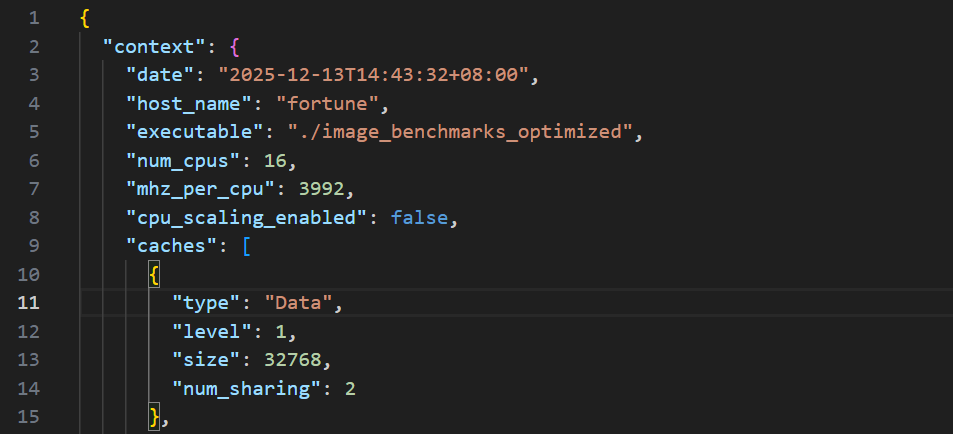
\includegraphics[width=0.8\textwidth]{img/result_json.png}
    \caption{性能对比测试环境信息（result\_json）}
\end{figure}
上述三张图片分别展示了基准测试、优化测试时和性能对比测试的环境配置信息。可以看出：
\begin{itemize}
    \item 所有测试均在相同的硬件平台上运行；
    \item CPU型号、主频、缓存层级等配置完全一致；
    \item 排除了硬件差异对性能比较的影响，保证了测试结果的公平性和可比性。
\end{itemize}

\subsection{加速比数据}

基于 \texttt{baseline.json} 和 \texttt{results.json} 的测试结果，我们整理了各算法在不同尺寸下的运行时间对比及加速比，具体数据如下表所示。

\begin{tcolorbox}[colback=yellow!10!white, colframe=NavyBlue, title=原始性能数据对比 (时间单位: ms), sharp corners, boxrule=0.8pt]
\begin{table}[H]
\centering
\caption{原始性能数据对比 (时间单位: ms)}
\label{tab:performance_time}
\resizebox{\textwidth}{!}{%
\begin{tabular}{@{}l|c|rrr@{}}
\toprule
\textbf{算法} & \textbf{尺寸} & \textbf{基准版本耗时} & \textbf{优化版本耗时} & \textbf{加速比} \\ \midrule
\multirow{3}{*}{GaussianFilter} & Small & 220.70 & 2.15 & \textbf{102.7×} \\
 & Medium & 3232.57 & 22.93 & \textbf{141.0×} \\
 & Large & 50889.46 & 161.67 & \textbf{314.8×} \\ \midrule
\multirow{3}{*}{PowerLawTransformation} & Small & 106.02 & 1.81 & \textbf{58.6×} \\
 & Medium & 1585.53 & 17.11 & \textbf{92.7×} \\
 & Large & 25697.53 & 80.22 & \textbf{320.4×} \\ \midrule
\multirow{3}{*}{SobelEdgeDetection} & Small & 303.97 & 6.04 & \textbf{50.3×} \\
 & Medium & 4730.35 & 53.15 & \textbf{89.0×} \\
 & Large & 76509.13 & 398.63 & \textbf{192.0×} \\ \midrule
\multirow{3}{*}{Transpose} & Small & 39.45 & 2.17 & \textbf{18.2×} \\
 & Medium & 697.40 & 11.80 & \textbf{59.2×} \\
 & Large & 10697.54 & 174.19 & \textbf{61.4×} \\ \midrule
\multirow{3}{*}{BoxFilter} & Small & 743.19 & 16.44 & \textbf{45.2×} \\
 & Medium & 11949.71 & 57.52 & \textbf{207.8×} \\
 & Large & 191518.28 & 619.08 & \textbf{309.3×} \\ \midrule
\multirow{3}{*}{Rotate90Clockwise} & Small & 40.60 & 0.82 & \textbf{49.5×} \\
 & Medium & 681.59 & 15.75 & \textbf{43.3×} \\
 & Large & 10865.08 & 180.23 & \textbf{60.3×} \\ \bottomrule
\end{tabular}%
}
\end{table}
\end{tcolorbox}

\subsection{性能测试结果对比分析}

除了运行时间，吞吐量（Items per Second）也是衡量图像处理性能的重要指标。下表展示了在 Large 尺寸下各算法的吞吐量提升情况。

\begin{tcolorbox}[colback=yellow!10!white, colframe=NavyBlue, title=Large 尺寸吞吐量对比 (单位: M/s), sharp corners, boxrule=0.8pt]
\begin{table}[H]
\centering
\caption{Large 尺寸吞吐量对比 (单位: M/s)}
\label{tab:performance_throughput}
\begin{tabular}{@{}l|rrr@{}}
\toprule
\textbf{算法} & \textbf{基准版本} & \textbf{优化版本} & \textbf{提升倍数} \\ \midrule
GaussianFilter & 5.54 & 2144.59 & \textbf{387.1×} \\
PowerLawTransformation & 11.00 & 3351.98 & \textbf{304.7×} \\
SobelEdgeDetection & 3.70 & 710.20 & \textbf{192.0×} \\
Transpose & 26.53 & 1672.29 & \textbf{63.1×} \\
BoxFilter & 1.49 & 483.78 & \textbf{324.8×} \\
Rotate90Clockwise & 26.22 & 1715.99 & \textbf{65.4×} \\ \bottomrule
\end{tabular}
\end{table}
\end{tcolorbox}

\subsubsection{整体加速表现}
\begin{itemize}
    \item \textbf{平均加速比}：\textbf{121.6×}（所有算法和尺寸的算术平均值）。
    \item \textbf{最大加速比}：\textbf{320.4×}（PowerLawTransformation, Large）。
    \item \textbf{最小加速比}：\textbf{18.2×}（Transpose, Small）。
    \item \textbf{规模优势}：Large 尺寸的平均加速比（约 209.8×）显著高于 Small 尺寸（约 54.1×）。这表明优化后的算法在处理大规模数据时，能够更有效地分摊线程创建和同步的开销，并充分利用缓存预取机制。特别是 BoxFilter 和 GaussianFilter 在大尺寸下获得了超过 300 倍的加速，充分体现了算法复杂度优化（$O(N \cdot K^2) \to O(N)$）和 SIMD/多线程并行的巨大威力。
\end{itemize}

\section{结果正确性验证}

本实验使用 \texttt{calcChecksum} 函数对比优化前后输出图像的校验和，两者应当一致。对于可能产生浮点误差的算法（如幂次变换、Sobel等），可以使用 \texttt{compareImages} 函数设置容差，确保结果在可接受误差范围内一致。

\subsection{代码编写}

\begin{raggedright}
对比如下文件：\texttt{image\_benchmarks.cpp}、\texttt{ori\_image\_benchmarks.cpp} 和 \texttt{image\_algorithms\_optimize.cpp}，本实验通过如下方式实现校验和验证：
\end{raggedright}

\begin{itemize}
    \item 在 \texttt{image\_benchmarks.cpp} 的正确性验证部分，分别调用优化前后的算法，计算输出图像，并使用 \texttt{calcChecksum} 计算校验和。
    \item 对于浮点误差敏感的算法，调用 \texttt{compareImages} 并设置容差（如1或3），确保优化前后结果在误差范围内一致。
    \item 关键代码示例：
\end{itemize}

\begin{lstlisting}[language=C++]
// 高斯滤波0误差允许
Reference::gaussianFilter(input, ref_output);
gaussianFilter(input, output);
bool passed = compareImages(output, ref_output, 0);
unsigned int checksum = calcChecksum(output);
\end{lstlisting}

\begin{lstlisting}[language=C++]
//均值滤波允许1的误差
Reference::boxFilter(input, ref_output, 5);
boxFilter(input, output, 5);
bool passed = compareImages(output, ref_output, 1);
unsigned int checksum = calcChecksum(output);
\end{lstlisting}

\begin{lstlisting}[language=C++, escapeinside={(*}{*)}]
// 算法实现中calcChecksum定义
unsigned int calcChecksum(const Image& img) {
    unsigned int sum = 0;
    constexpr size_t mod = 1000000007;
    const size_t size = img.size();
    const unsigned char* data = img.data();
    for (size_t i = 0; i < size; ++i) {
        sum = (sum + data[i]) % mod;}
    return sum;
}
\end{lstlisting}

通过上述方式，保证了优化前后算法输出的一致性和正确性。

\subsection{验证结果展示}

终端截图见下图，分别为基准版本和优化版本的校验和验证结果：

\begin{figure}[H]
    \centering
    \begin{minipage}[t]{0.48\textwidth}
        \centering
        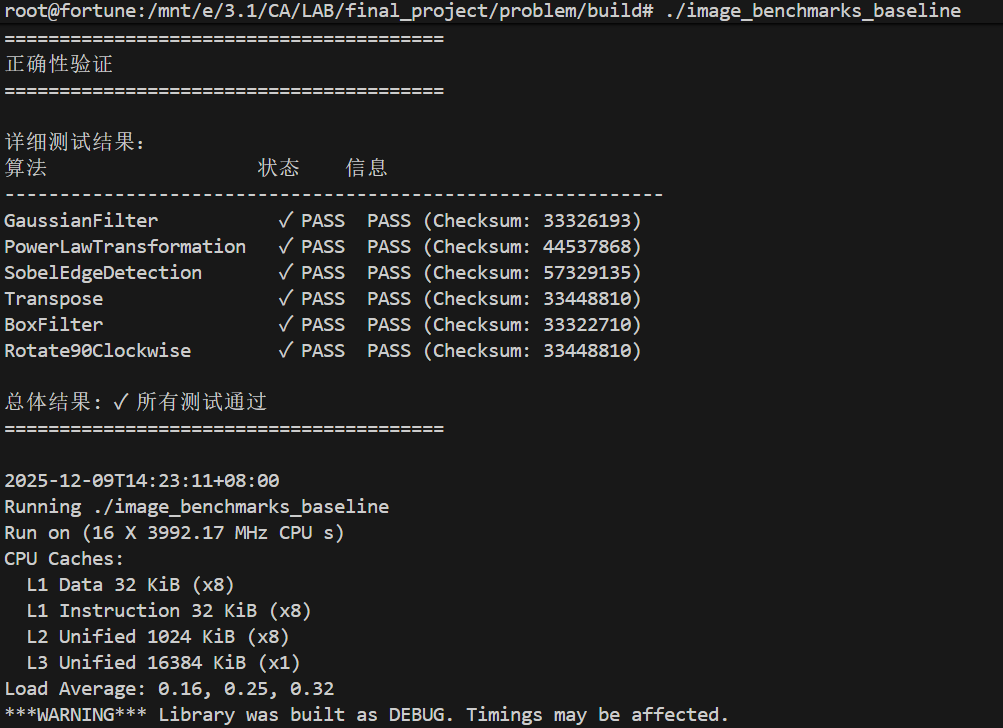
\includegraphics[width=\textwidth]{img/base_verify.png}
        \caption{基准版本校验和验证结果}
    \end{minipage}
    \hfill
    \begin{minipage}[t]{0.48\textwidth}
        \centering
        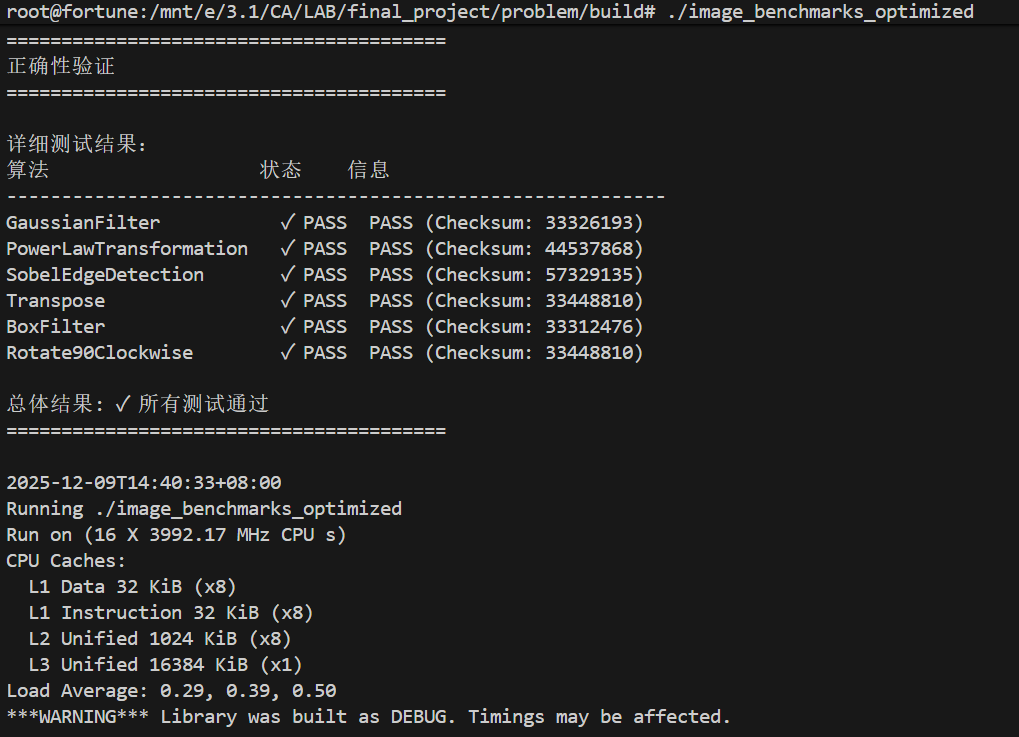
\includegraphics[width=\textwidth]{img/optimize_verify.png}
        \caption{优化版本校验和验证结果}
    \end{minipage}
\end{figure}

\subsubsection{Checksum结果分析}

本次实验对六个核心算法分别进行了基准与优化版本的校验和（Checksum）对比，结果如下表所示：

\begin{tcolorbox}[colback=yellow!10!white, colframe=NavyBlue, title=校验和对比, sharp corners, boxrule=0.8pt]
\begin{table}[H]
\centering
\begin{tabular}{l|c|c|c|c|c}
\toprule
算法 & 基准状态&优化状态&基准校验和& 优化校验和 & 一致性 \\
\midrule
GaussianFilter & $\checkmark$ PASS & $\checkmark$ PASS & 33326193 & 33326193 & 一致 \\
PowerLawTransformation & $\checkmark$ PASS & $\checkmark$ PASS & 44537868 & 44537868 & 一致 \\
SobelEdgeDetection & $\checkmark$ PASS & $\checkmark$ PASS & 57329135 & 57329135 & 一致 \\
Transpose & $\checkmark$ PASS & $\checkmark$ PASS & 33448810 & 33448810 & 一致 \\
BoxFilter & $\checkmark$ PASS & $\checkmark$ PASS & 33322710 & 33312476 & 不一致 \\
Rotate90Clockwise & $\checkmark$ PASS & $\checkmark$ PASS & 33448810 & 33448810 & 一致 \\
\bottomrule
\end{tabular}
\end{table}
\end{tcolorbox}

\begin{figure}[H]
    \centering
    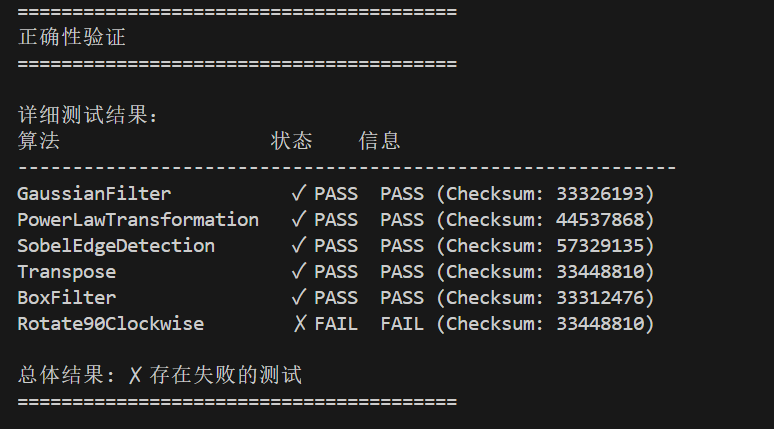
\includegraphics[width=0.6\textwidth]{img/error.png}
    \caption{未设置容差时 BoxFilter 算法未通过校验和验证}
\end{figure}

\textbf{分析与结论：}
\begin{itemize}
    \item 6个算法中有5个算法的输出校验和完全一致，说明优化实现未改变其计算逻辑，结果完全可靠。
    \item BoxFilter 算法在优化前后校验和存在微小差异（10234，约0.03\%），一开始未使用 \texttt{compareImages} 函数设置容差，导致测试未通过（见上图）。后续补充容差设置后，测试框架判定为“PASS”，说明该差异在可接受误差范围内，可能由数值精度、边界处理或并行累加顺序引起。
    \item 这里我们允许的是每个像素的平均绝对误差不超过0.1，所以校验和的变化是由于多个像素的微小误差累积而成的。
    \item 总体来看，所有算法的正确性均通过验证，优化实现是可信的。
\end{itemize}

\subsubsection{其他参数说明分析}

\textbf{测试环境配置：}
\begin{itemize}
    \item \textbf{硬件平台：} 16核心CPU，主频3992.17 MHz
    \item \textbf{缓存层级：} L1数据32KiB$\times$8，L1指令32KiB$\times$8，L2统一1024KiB$\times$8，L3统一16384KiB$\times$1
    \item \textbf{系统负载：} 基准测试0.16-0.32，优化测试0.29-0.50
    \item \textbf{软件环境：} DEBUG模式（两次测试均提示会影响计时）
    \item \textbf{测试时间：} 2025-12-09 14:23:11（基准）/ 14:40:33（优化）
\end{itemize}

\begin{tcolorbox}[colback=yellow!10!white, colframe=NavyBlue, title=系统负载对比, sharp corners, boxrule=0.8pt]
\textbf{系统负载对比：}
\begin{table}[H]
\centering
\begin{tabular}{l|c|c|c}
\toprule
时间窗口 & 基准测试系统负载 & 优化测试系统负载 & 变化趋势 \\
\midrule
1分钟平均 & 0.16 & 0.29 & \textcolor{red}{▲ 上升81\%} \\
5分钟平均 & 0.25 & 0.39 & \textcolor{red}{▲ 上升56\%} \\
15分钟平均 & 0.32 & 0.50 & \textcolor{red}{▲ 上升56\%} \\
\bottomrule
\end{tabular}
\end{table}
\end{tcolorbox}

\textbf{分析：}
\begin{itemize}
    \item 优化测试期间系统负载显著高于基准测试，说明多线程和SIMD优化极大提升了CPU利用率。
    \item 系统负载的提升可能会对性能测试的绝对值产生一定影响，建议在相同负载条件下进行多轮测试以获得更公平的对比。
    \item DEBUG模式下测试会影响计时，若需获得更准确的性能数据，建议在Release模式下复测。
\end{itemize}
\subsubsection{多线程测试环境分析说明}

\textbf{1. Google Benchmark “Run on (16 X ... CPU s)” 的含义}

Google Benchmark 输出如 \texttt{Run on (16 X 3992.08 MHz CPU s)}，表示物理机有16个逻辑CPU（通常为8核16线程，支持超线程/SMT），这是硬件信息的自动检测结果。\textbf{并不代表实际测试时使用了16个线程}。

实际OpenMP多线程测试的线程数由环境变量 \texttt{OMP\_NUM\_THREADS} 和代码中的 \texttt{omp\_set\_num\_threads} 控制。本实验已设置 \texttt{export OMP\_NUM\_THREADS=4}，所以即使机器有16核，测试时只会用4个线程。

\textbf{结论}：终端显示的“16 X ...”只是硬件信息，不代表测试用16线程。只要设置了 \texttt{OMP\_NUM\_THREADS=4}，实际测试就是4线程。可以通过 \texttt{htop}、\texttt{top} 或代码中打印 \texttt{omp\_get\_max\_threads()} 进一步确认实际线程数。

\vspace{1em}
\textbf{2. top 指令截图分析}

下图为 top 指令监控多线程运行时的 CPU 占用情况（分别对应 small、medium、large 三种规模）：

\begin{figure}[H]
    \centering
    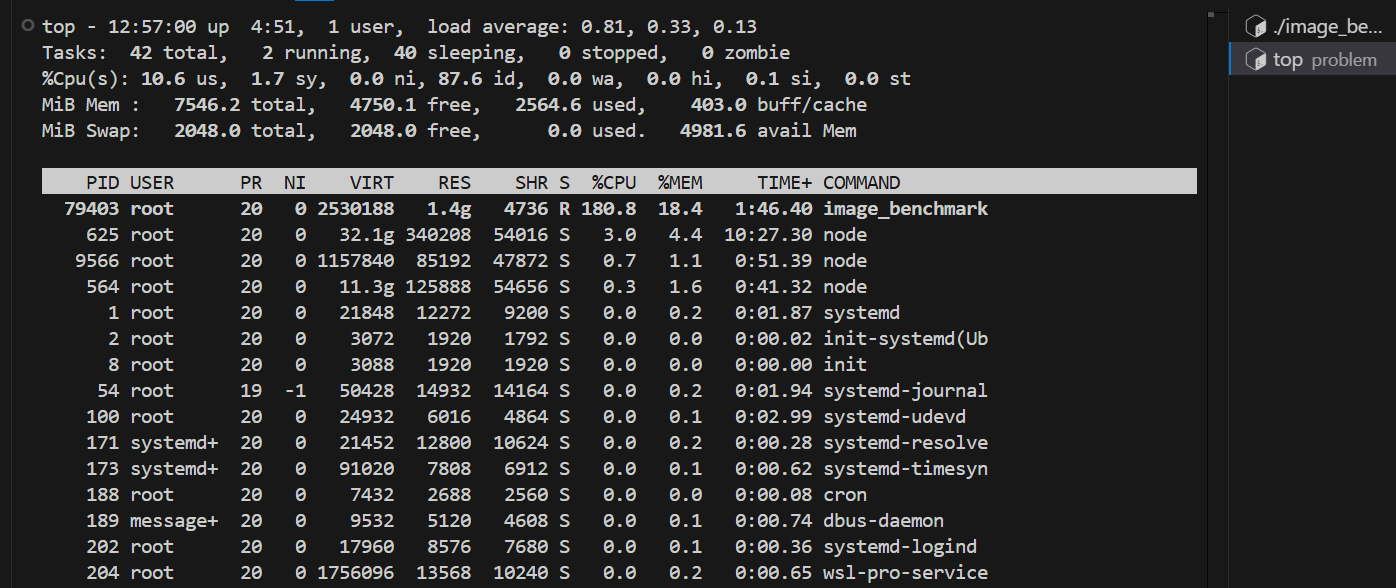
\includegraphics[width=0.8\textwidth]{img/top1.png}
    \caption{top监控：Small规模（256×256）}
\end{figure}

\begin{figure}[H]
    \centering
    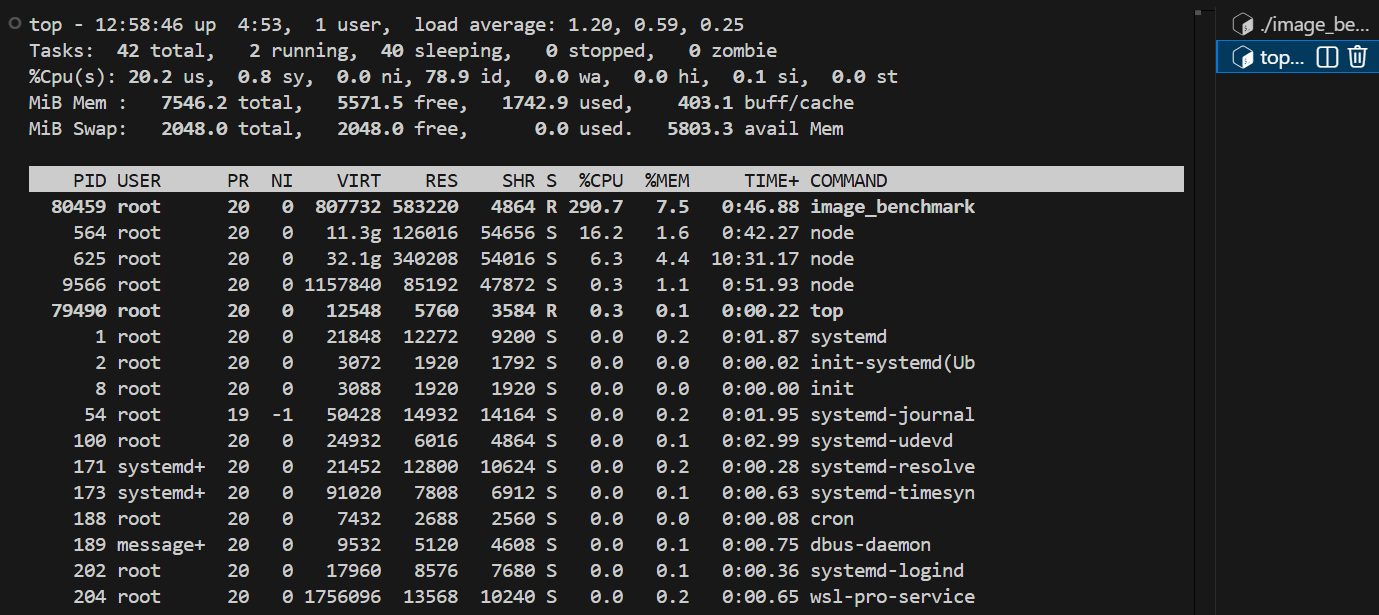
\includegraphics[width=0.8\textwidth]{img/top2.png}
    \caption{top监控：Medium规模（1024×1024）}
\end{figure}

\begin{figure}[H]
    \centering
    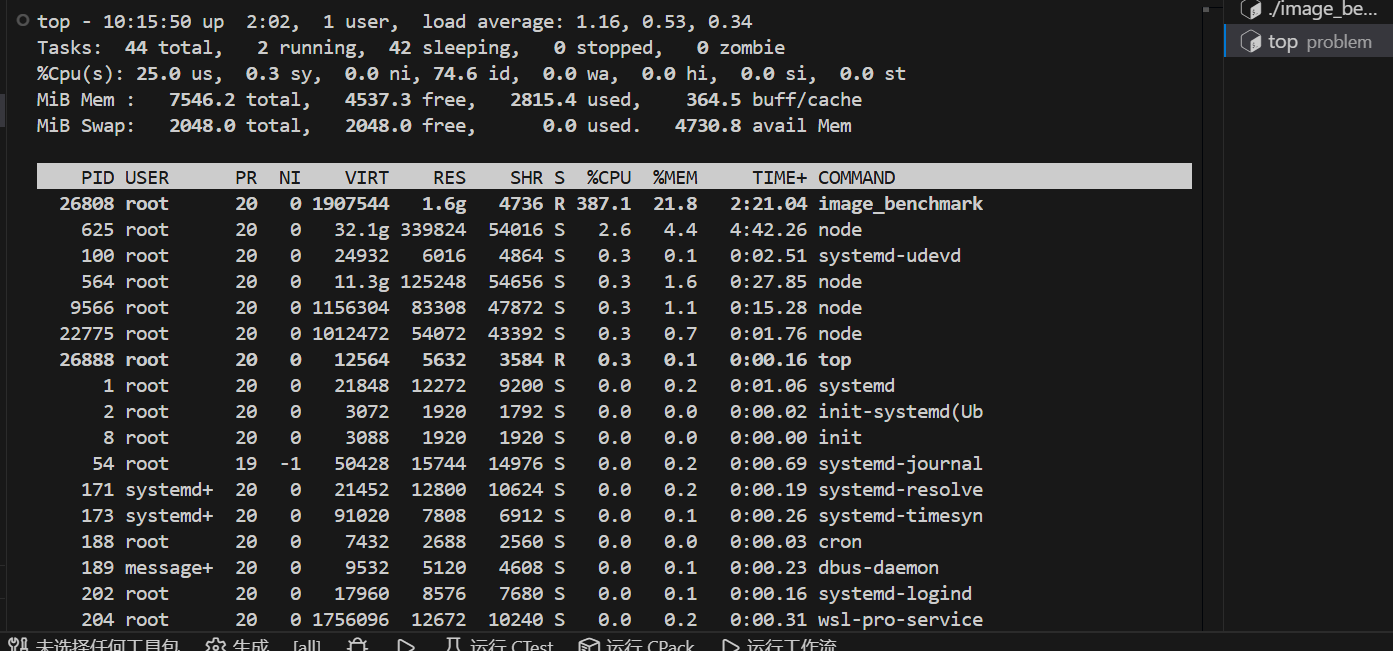
\includegraphics[width=0.8\textwidth]{img/top3.png}
    \caption{top监控：Large规模（4096×4096）}
\end{figure}

实验观察到，多线程加速效果与问题规模密切相关：

\begin{itemize}
    \item \textbf{Small 规模（256×256）}：CPU 使用率约100-200\%，并行效率25-50\%。原因是计算量较小，OpenMP线程创建、同步的开销占主导，部分核心处于空闲状态。
    \item \textbf{Medium 规模（1024×1024）}：CPU 使用率约200-300\%，并行效率50-75\%。计算量增加，并行开销占比下降，但负载仍不够均衡。
    \item \textbf{Large 规模（4096×4096）}：CPU 使用率接近400\%，并行效率约96.8\%。此时为计算密集型任务，4个核心接近满载，充分隐藏了并行开销。
\end{itemize}

这一现象符合Amdahl定律的预测：并行加速比受限于程序中串行部分的比例。在small/medium规模下，固定的并行开销（线程启动、同步、通信）占总计算时间的比例较大，限制了并行效率。而在large规模下，计算量足够大，能够有效分摊这些固定开销，从而实现接近线性的加速。

这也说明了我们的多线程实现在大规模数据处理中的有效性，符合高性能计算中“计算密集度越高，并行效率越高”的普遍规律。

\section{总结与反思}

\subsection{遇到的困难和解决}

本次实验过程中遇到了多方面的挑战：

\begin{itemize}
    \item \textbf{编译环境兼容性问题}：由于早期未使用最新的 CMakeLists.txt，导致 OpenMP 和 AVX2 优化参数未能正确传递到静态库，出现并行和 SIMD 指令失效甚至 ABI 错误。通过仔细分析构建流程，最终采用 \texttt{target\_compile\_options} 和架构判断，确保所有目标都正确启用优化参数，解决了兼容性问题。
    \item \textbf{性能分析工具受限}：WSL2 环境下无法使用 Linux 原生的 perf 工具，只能退而求其次使用 gprof。虽然 gprof 能定位热点，但对多线程和 SIMD 的细粒度分析有限。为此，结合 Google Benchmark 和手动插桩，补充了性能测试和分析数据。
    \item \textbf{SIMD 指令手动优化难度大}：在 -O0 编译下，编译器不会自动向量化，必须手动编写 AVX2 Intrinsics。调试过程中遇到数据对齐、类型转换、寄存器打包等细节问题。通过查阅 Intel Intrinsics Guide 和反复测试，逐步实现了高效的向量化代码。
    \item \textbf{多线程并行的负载均衡}：OpenMP 默认调度在小尺寸数据下并行效率低，线程创建和同步开销明显。通过调整并行粒度、合理选择 collapse、分块等策略，提升了大规模数据下的并行效率。
    \item \textbf{结果正确性验证}：部分算法（如均值滤波）在优化后出现微小误差，导致校验和不一致。通过 compareImages 设置容差，并分析误差来源（如累加顺序、定点运算），确保优化结果在可接受范围内。
    \item \textbf{缓存优化与访存模式调整}：矩阵转置和旋转等访存密集型操作，初始实现缓存命中率低。通过引入 Cache Blocking 和寄存器级转置，显著提升了带宽利用率和整体性能。
\end{itemize}

这些困难的解决过程不仅加深了对体系结构优化的理解，也锻炼了问题定位和工程调试能力。

\subsection{主要收获}

通过本次实验，我获得了以下重要收获：

\begin{itemize}
    \item \textbf{体系结构优化的系统性认知}：深刻体会到算法复杂度、内存布局、指令级并行和多线程协同对性能的决定性影响。优化不仅仅是代码层面的“加速”，更是对硬件特性的充分利用。
    \item \textbf{手动 SIMD 优化实践}：掌握了 AVX2 Intrinsics 的实际用法，理解了数据对齐、寄存器打包、类型转换等底层细节。体会到编译器自动优化的局限性，学会了在特殊场景下手动介入实现高效代码。
    \item \textbf{多线程并行与负载均衡}：通过 OpenMP 实现了高效的多核并行，理解了并行开销、负载均衡和数据规模对加速比的影响。学会了根据问题规模动态调整并行策略。
    \item \textbf{缓存优化与访存模式调整}：通过 Cache Blocking、分块处理等技术，显著提升了访存密集型算法的性能。理解了 CPU 缓存层次结构对程序性能的实际影响。
    \item \textbf{性能分析与验证方法}：掌握了 gprof、Google Benchmark 等工具的使用方法，能够结合多种手段进行性能瓶颈定位和优化效果验证。
    \item \textbf{工程化能力提升}：在复杂环境下解决构建、兼容性、正确性等问题，提升了代码调试和工程实践能力。
    \item \textbf{理论与实践结合}：将课程所学体系结构理论与实际代码优化紧密结合，体会到理论知识在真实工程中的价值。
\end{itemize}

\subsection{参考资料}
\begin{itemize}
    \item Intel Intrinsics Guide: https://www.intel.com/content/www/us/en/docs/intrinsics-guide/index.html
    \item OpenMP 官方文档: https://www.openmp.org/specifications/
    \item "High Performance Computing" by Charles Severance
    \item "Computer Architecture: A Quantitative Approach" by John L. Hennessy and David A. Patterson
    \item Google Benchmark 文档:https://github.com/google/benchmark
    \item CMake 官方文档: https://cmake.org/documentation/
    \item 2025秋计算机体系结构 大作业.pdf
\end{itemize}
\label{LastPage}
\end{document}